% figures/timing-methods.tex
% The three timing methods of the performance campaign, in increasing
% isolation of the GPU kernel.
\documentclass[tikz,border=10pt]{standalone}
% figures/common-preamble.tex
% Shared setup for the TikZ documentation figures. Colors mirror the
% palette in scripts/render_docs_diagrams.py so both atlases match.
\usepackage[T1]{fontenc}
\usepackage{lmodern}
\usepackage{tikz}
\usepackage{pgfplots}
\pgfplotsset{compat=1.18}
\usetikzlibrary{arrows.meta}
\usetikzlibrary{backgrounds}
\usetikzlibrary{calc}
\usetikzlibrary{decorations.pathreplacing}
\usetikzlibrary{fit}
\usetikzlibrary{positioning}

\definecolor{swcanvas}{HTML}{FFFDF8}
\definecolor{swpanel}{HTML}{F5F3ED}
\definecolor{swink}{HTML}{17212B}
\definecolor{swmuted}{HTML}{4B5563}
\definecolor{swline}{HTML}{59636E}
\definecolor{swblue}{HTML}{00689D}
\definecolor{swbluefill}{HTML}{DCEFFD}
\definecolor{swpurple}{HTML}{8E4775}
\definecolor{swpurplefill}{HTML}{F7E2EF}
\definecolor{sworange}{HTML}{A94500}
\definecolor{sworangefill}{HTML}{FCE5DC}
\definecolor{swgreen}{HTML}{00664B}
\definecolor{swgreenfill}{HTML}{DDF4EB}
\definecolor{swgrayfill}{HTML}{EEF0F2}

\pagecolor{swcanvas}
\AtBeginDocument{\color{swink}}

\tikzset{
  swcell/.style={
    draw, minimum width=0.46cm, minimum height=0.46cm, inner sep=0pt,
    line width=0.7pt, rounded corners=1pt},
  swbox/.style={
    draw=swline, fill=swpanel, rounded corners=6pt, line width=0.9pt},
  swarrow/.style={-{Stealth[length=6pt]}, draw=swline, line width=1pt},
  swtag/.style={
    draw, rounded corners=8pt, line width=0.9pt,
    font=\bfseries\scriptsize, inner xsep=8pt, inner ysep=4pt},
  swtitle/.style={anchor=west, font=\Large\bfseries, text=swink},
  swsubtitle/.style={anchor=west, font=\small, text=swmuted},
  swcode/.style={font=\small\ttfamily, text=swink},
  every picture/.style={line cap=round},
}

\begin{document}
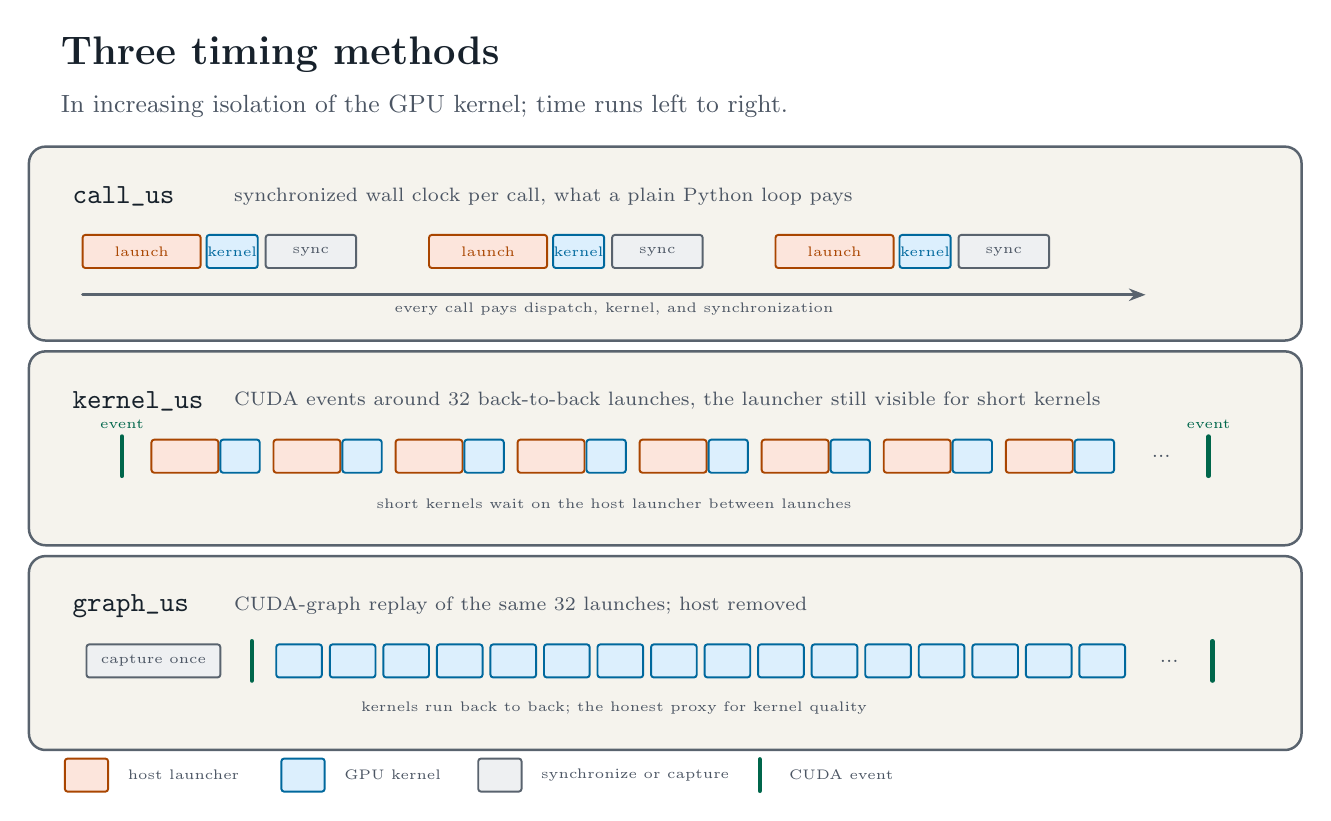
\begin{tikzpicture}[x=1cm, y=1cm,
  host/.style={swcell, fill=sworangefill, draw=sworange,
    minimum height=0.42cm, rounded corners=1pt},
  kern/.style={swcell, fill=swbluefill, draw=swblue,
    minimum height=0.42cm, rounded corners=1pt},
  sync/.style={swcell, fill=swgrayfill, draw=swline,
    minimum height=0.42cm, rounded corners=1pt},
  evmark/.style={draw=swgreen, line width=1.6pt}]

% Header.
\node[swtitle] at (0, 1.15) {Three timing methods};
\node[swsubtitle] at (0, 0.5)
  {In increasing isolation of the GPU kernel; time runs left to
   right.};

% ------------------------------------------------------------ call_us
\node[swbox, fit={(0, -2.2) (15.6, -0.3)}, inner sep=8pt] {};
\node[anchor=west, font=\bfseries\ttfamily, text=swink]
  at (0.15, -0.65) {\detokenize{call_us}};
\node[anchor=west, font=\scriptsize, text=swmuted] at (2.2, -0.65)
  {synchronized wall clock per call, what a plain Python loop pays};
\foreach \r in {0, 1, 2} {
  \node[host, minimum width=1.5cm] at ({1.15 + \r * 4.4}, -1.35) {};
  \node[font=\tiny, text=sworange] at ({1.15 + \r * 4.4}, -1.35)
    {launch};
  \node[kern, minimum width=0.65cm] at ({2.3 + \r * 4.4}, -1.35) {};
  \node[font=\tiny, text=swblue] at ({2.3 + \r * 4.4}, -1.35) {kernel};
  \node[sync, minimum width=1.15cm] at ({3.3 + \r * 4.4}, -1.35) {};
  \node[font=\tiny, text=swmuted] at ({3.3 + \r * 4.4}, -1.35) {sync};
}
\draw[swarrow] (0.4, -1.9) -- (13.9, -1.9);
\node[font=\tiny, text=swmuted] at (7.15, -2.08)
  {every call pays dispatch, kernel, and synchronization};

% ---------------------------------------------------------- kernel_us
\node[swbox, fit={(0, -4.8) (15.6, -2.9)}, inner sep=8pt] {};
\node[anchor=west, font=\bfseries\ttfamily, text=swink]
  at (0.15, -3.25) {\detokenize{kernel_us}};
\node[anchor=west, font=\scriptsize, text=swmuted] at (2.2, -3.25)
  {CUDA events around 32 back-to-back launches,
   the launcher still visible for short kernels};
\draw[evmark] (0.9, -4.2) -- (0.9, -3.7);
\node[font=\tiny, text=swgreen] at (0.9, -3.55) {event};
\foreach \r in {0,...,7} {
  \node[host, minimum width=0.85cm] at ({1.7 + \r * 1.55}, -3.95) {};
  \node[kern, minimum width=0.5cm] at ({2.4 + \r * 1.55}, -3.95) {};
}
\node[font=\scriptsize, text=swmuted] at (14.1, -3.95) {...};
\draw[evmark] (14.7, -4.2) -- (14.7, -3.7);
\node[font=\tiny, text=swgreen] at (14.7, -3.55) {event};
\node[font=\tiny, text=swmuted] at (7.15, -4.55)
  {short kernels wait on the host launcher between launches};

% ----------------------------------------------------------- graph_us
\node[swbox, fit={(0, -7.4) (15.6, -5.5)}, inner sep=8pt] {};
\node[anchor=west, font=\bfseries\ttfamily, text=swink]
  at (0.15, -5.85) {\detokenize{graph_us}};
\node[anchor=west, font=\scriptsize, text=swmuted] at (2.2, -5.85)
  {CUDA-graph replay of the same 32 launches; host removed};
\node[sync, minimum width=1.7cm] at (1.3, -6.55) {};
\node[font=\tiny, text=swmuted] at (1.3, -6.55) {capture once};
\draw[evmark] (2.55, -6.8) -- (2.55, -6.3);
\foreach \r in {0,...,15} {
  \node[kern, minimum width=0.58cm] at ({3.15 + \r * 0.68}, -6.55) {};
}
\node[font=\scriptsize, text=swmuted] at (14.2, -6.55) {...};
\draw[evmark] (14.75, -6.8) -- (14.75, -6.3);
\node[font=\tiny, text=swmuted] at (7.15, -7.15)
  {kernels run back to back; the honest proxy for kernel quality};

% Legend.
\node[host, minimum width=0.55cm] at (0.45, -8.0) {};
\node[anchor=west, font=\tiny, text=swmuted] at (0.85, -8.0)
  {host launcher};
\node[kern, minimum width=0.55cm] at (3.2, -8.0) {};
\node[anchor=west, font=\tiny, text=swmuted] at (3.6, -8.0)
  {GPU kernel};
\node[sync, minimum width=0.55cm] at (5.7, -8.0) {};
\node[anchor=west, font=\tiny, text=swmuted] at (6.1, -8.0)
  {synchronize or capture};
\draw[evmark] (9.0, -8.2) -- (9.0, -7.8);
\node[anchor=west, font=\tiny, text=swmuted] at (9.25, -8.0)
  {CUDA event};

\end{tikzpicture}
\end{document}
